% Begin the document and set up the style of the document
\documentclass[a4paper]{article}

% Install the required packages for the document 
\usepackage{envmath}
\usepackage{esvect}
\usepackage{graphicx}
\usepackage{gensymb}
\usepackage{tikz}
\usepackage[mathcal]{euscript}
\usepackage{geometry}
\usepackage{enumitem}
\usepackage{mathtools}
\usepackage{subdepth}
\usepackage{graphicx}
\usepackage{amsmath}
\usepackage{amscd}
\usepackage{amssymb}
\usepackage{amsfonts}
\usepackage{harpoon}
\usepackage{pgf}
\usepackage{tikz}
\usepackage{mathrsfs}
\usepackage{asyalign}
\usepackage{physics}
\usepackage{enumitem}
\usepackage{xhfill}
\usepackage{accents}
\usepackage{cite}
\usepackage{url}
\usepackage{csquotes}
\usepackage{wrapfig}
\usepackage{booktabs}
\usepackage{adjustbox}
\usepackage{caption}
\usepackage{minipage-marginpar}
\usepackage{calc}
\usepackage[tableposition=top]{caption}
\usepackage{ifthen}
\usepackage[utf8]{inputenc}
\usepackage{tikz-3dplot}
\usetikzlibrary{patterns}
\usetikzlibrary{arrows}

% Page and style settings
\parskip=8pt
\parindent=0pt
% Right margin
\textwidth=6.25in
% Left margin
\oddsidemargin=0pt
\evensidemargin=0pt
% Bottom margin
\textheight=10in
% Top margin
\topmargin=-0.75in
\baselineskip=11pt
% end of page and other style settings

\renewcommand{\familydefault}{\sfdefault}

\newcommand{\indep}{\mathrel{\text{\scalebox{1.07}{$\perp\mkern-10mu\perp$}}}}
\newcommand{\p}{\mathbb{P}}
\newcommand{\e}{\mathbb{E}}
\newcommand{\ds}{\displaystyle}
\newcommand{\code}{\texttt}

% Begin the text of the document
\begin{document}

\newlength{\strutheight}
\settoheight{\strutheight}{\strut}

% Begin the Title Page
\begin{titlepage}

\newcommand{\HRule}{\rule{\linewidth}{0.5mm}} % Defines a new command for the horizontal lines, change thickness here

\center % Center everything on the page
 
\textsc{\LARGE University of New South Wales}\\[1.5cm] % Name of your university/college
\textsc{\Large MATH 2901}\\[0.5cm] % Major heading such as course name
\textsc{\large Higher Theory of Statistics}\\[0.5cm] % Minor heading such as course title

\HRule \\[0.4cm]
{ \huge \bfseries Assignment 2}\\[0.4cm] % Title of your document
\HRule \\[1.5cm]


\begin{center} \large
Keegan Gyoery (z5197058), John Lidbetter (z5160860),\\ 
Edward McInnes (z5162873), Alex Robinson (z5164884),\\ 
Ruby Smith (z5113171) % Your name
\\
\end{center}


\vspace{4cm}

{\today}\\[3cm] % Date, change the \today to a set date if you want to be precise

\vfill % Fill the rest of the page with whitespace

\end{titlepage}

\pagenumbering{arabic}

\begin{enumerate}

	\item $\ds{X_{1}}$ and $\ds{X_{2}}$ have the following density functions:
	\begin{align*}
		f_{X_1}(x) & = \frac{1}{x\sqrt{2\pi}}e^{-(\ln{x})^2/2} \hspace{5mm} x > 0 \\
		f_{X_2}(x) & = f_{X_1}(x)[1 + \sin(2\pi \ln{x})] \hspace{5mm} x > 0 \\
	\end{align*}
	\begin{enumerate}

		\item The graph for $\ds{f_{X_1}(x)}$ is shown in the following figure.
		\begin{figure}[h!]
			\begin{center}
				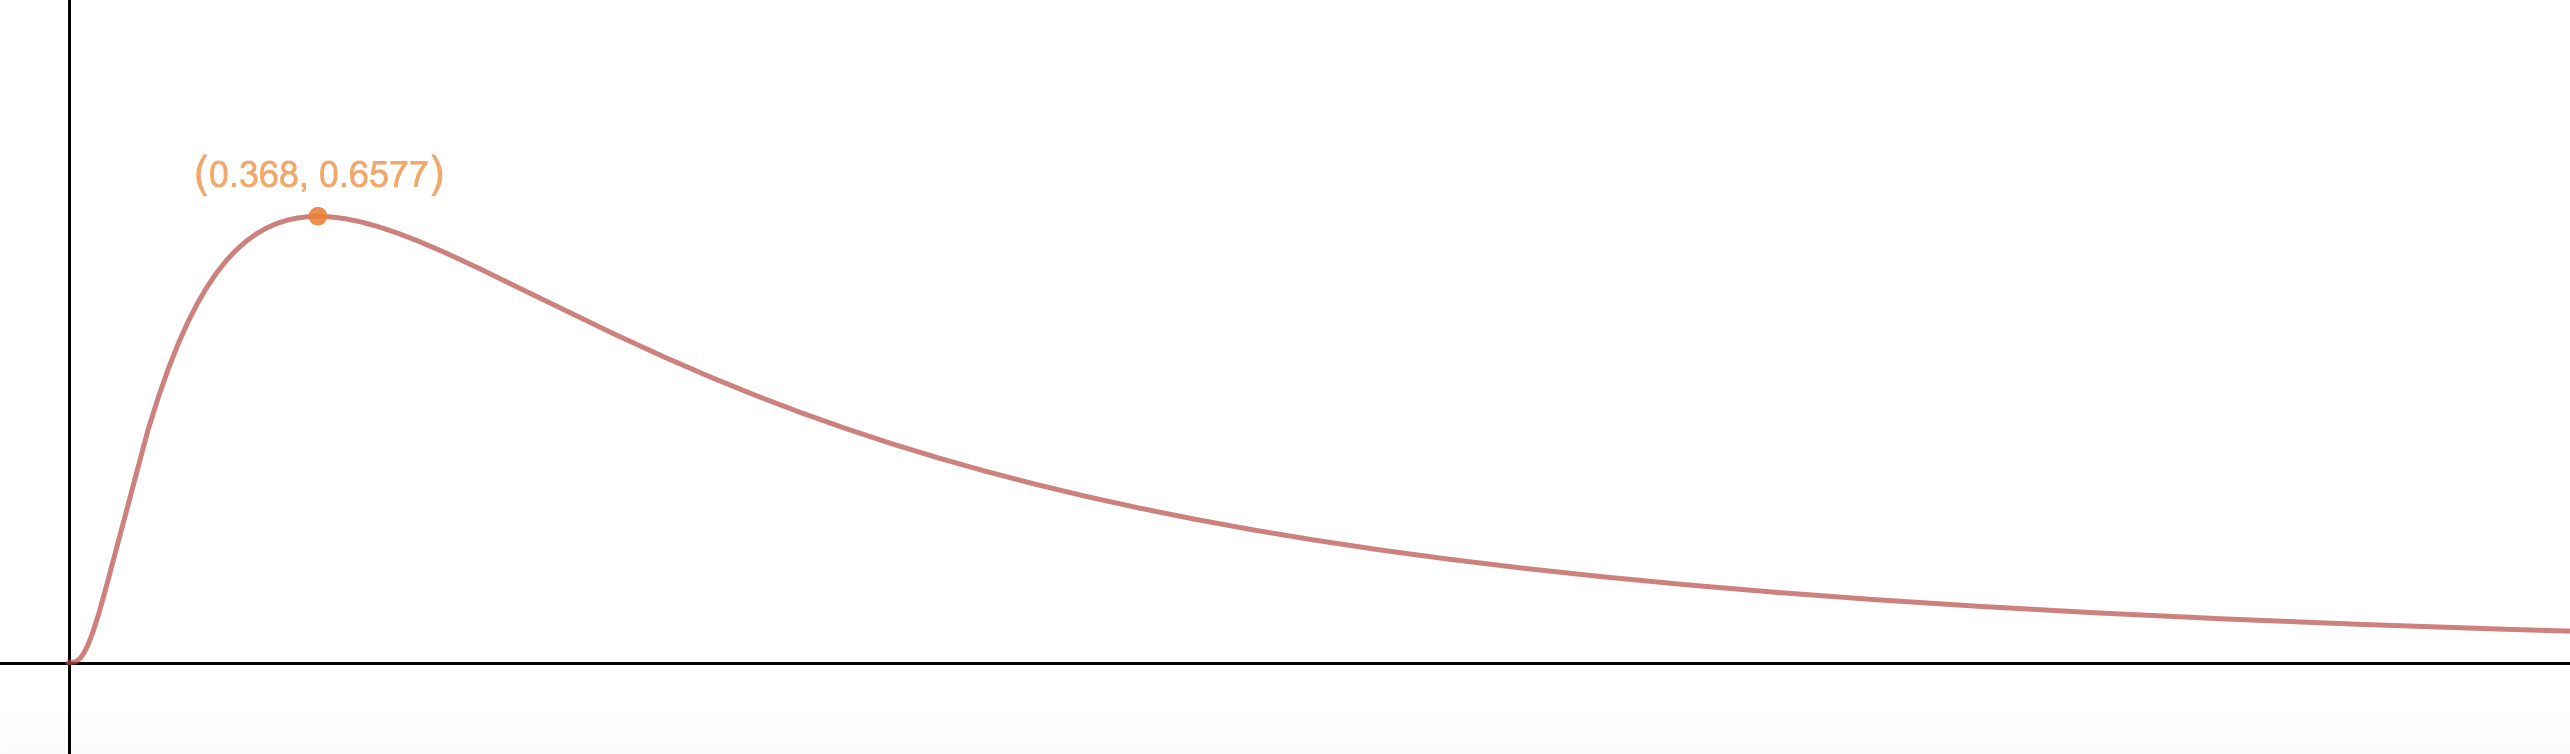
\includegraphics[width=0.6\linewidth]{12.png}
			\end{center}
		\end{figure}
		\bigbreak
		The max point occurs at $\ds{\bigg(\frac{1}{e},\sqrt{\frac{e}{2\pi}}\bigg)}$. As $\ds{x}$ approaches $\ds{0}$, $\ds{\ln x}$ approaches $\ds{-\infty}$. Thus, $\ds{e^{-(\ln{x})^2/2}}$ approaches $\ds{0}$. As $\ds{e^x}$ dominates $\ds{\frac{1}{x}}$, $\ds{f_{X_1}(x)}$ approaches $\ds{0}$ as $\ds{x}$ approaches $\ds{0}$. As $\ds{x}$ approaches $\ds{\infty}$, $\ds{\ln x}$ approaches $\ds{\infty}$. Thus, $\ds{e^{-(\ln{x})^2/2}}$ approaches $\ds{0}$. As $\ds{e^x}$ dominates $\ds{\frac{1}{x}}$, $\ds{f_{X_1}(x)}$ approaches $\ds{0}$ as $\ds{x}$ approaches $\ds{\infty}$.
		\bigbreak
		The graph for $\ds{f_{X_2}(x)}$ is shown in the following figure.
		\begin{figure}[h!]
			\begin{center}
				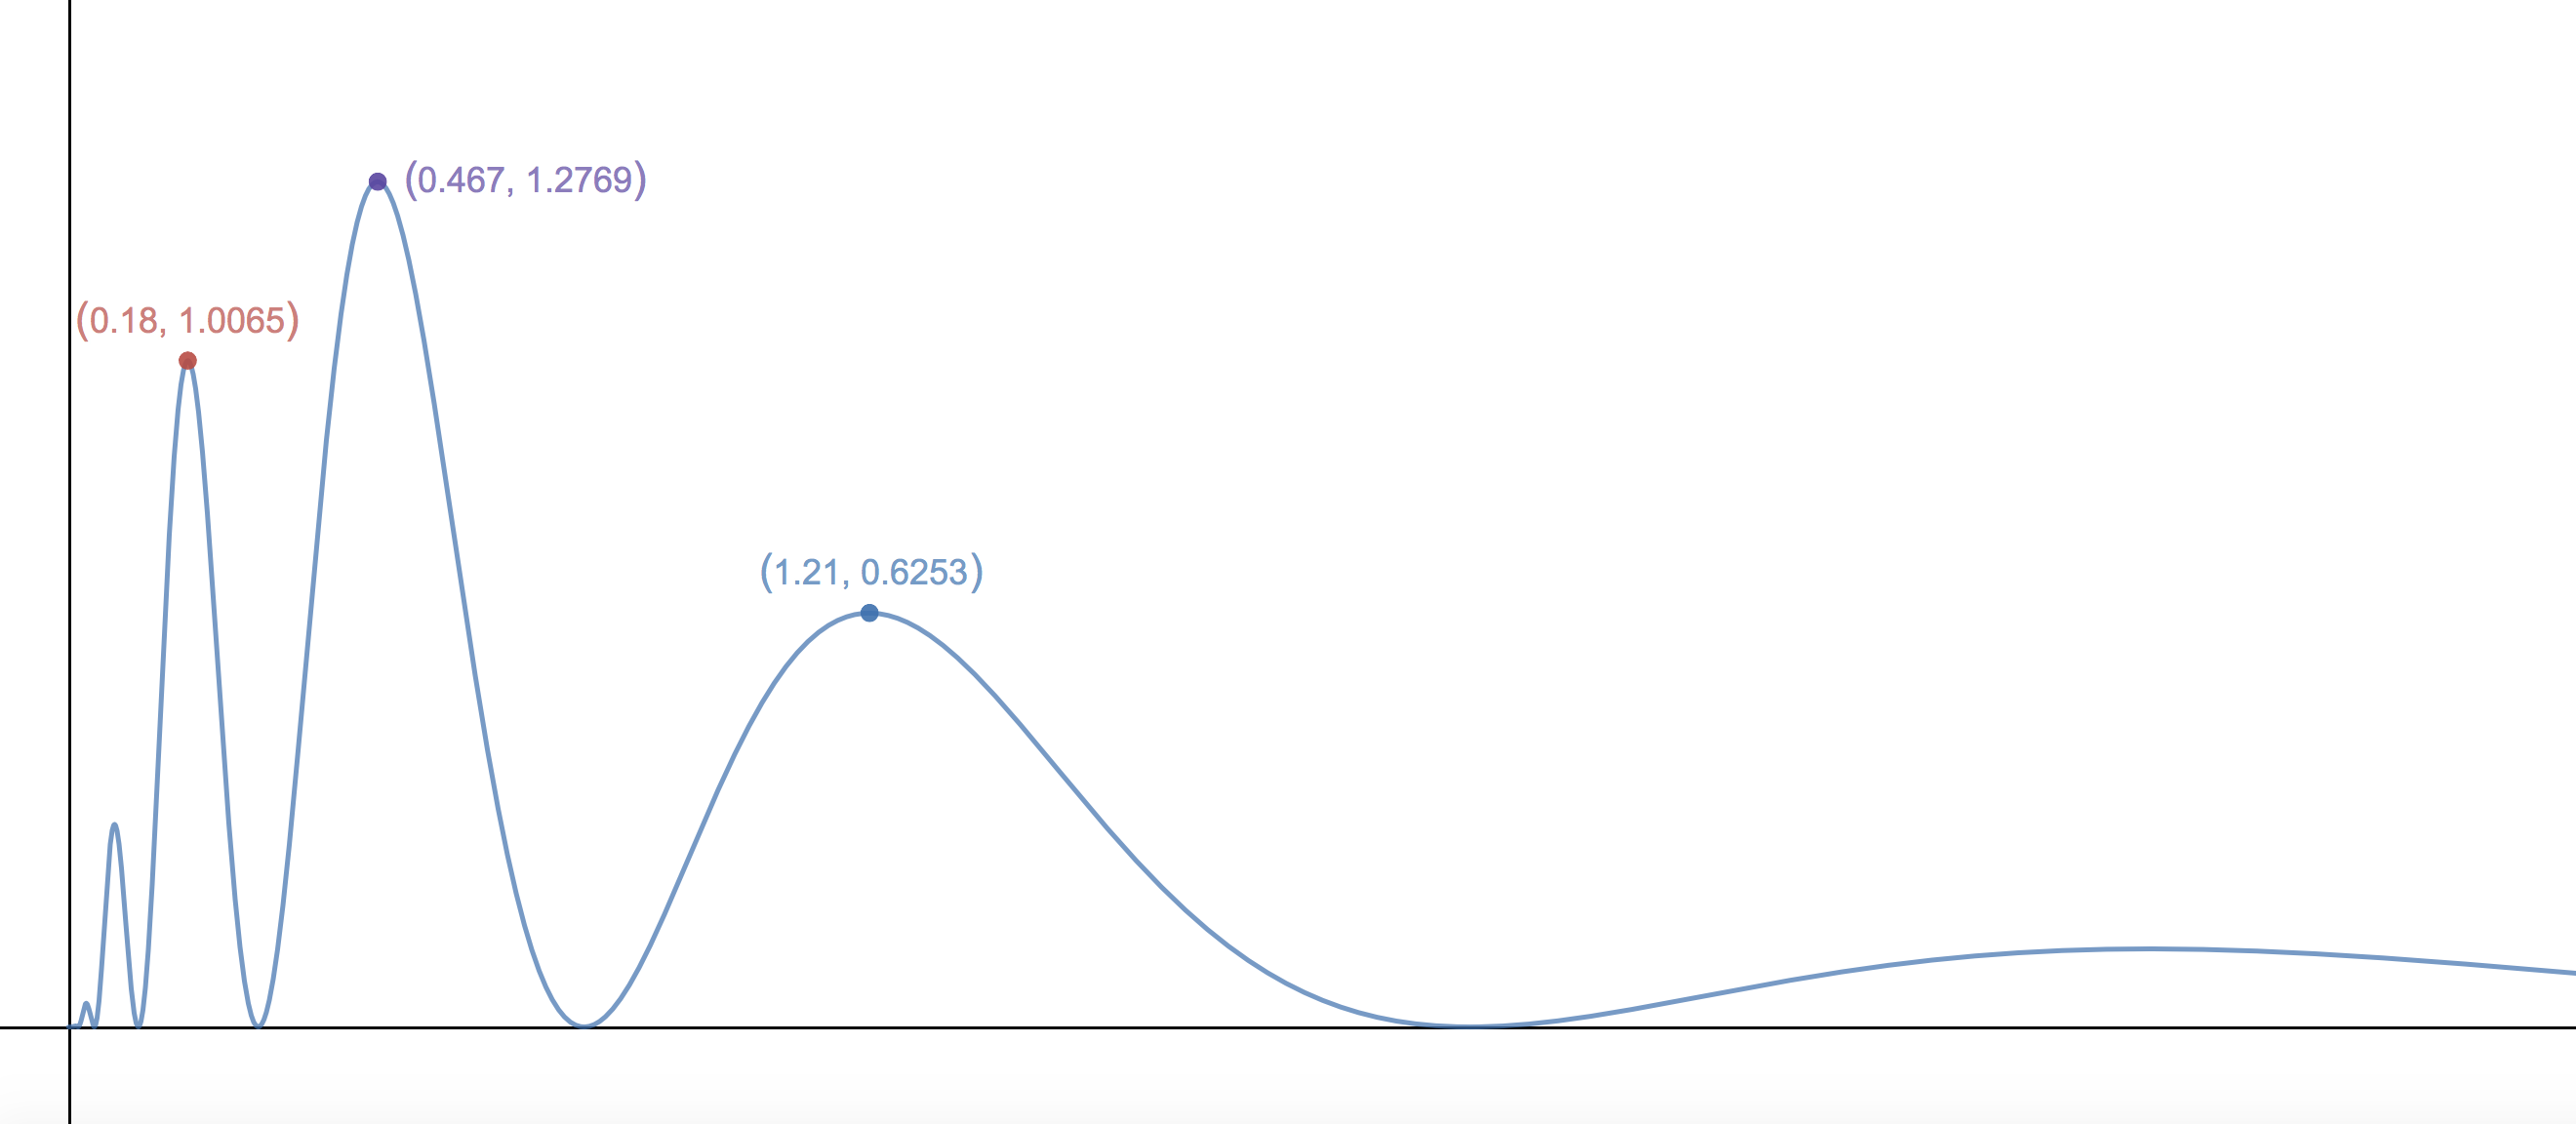
\includegraphics[width=0.6\linewidth]{22.png}
			\end{center}
		\end{figure}
		\bigbreak
		$\ds{f_{X_2}(x)}$ behaves in the same manner as $\ds{f_{X_1}(x)}$ when $\ds{x}$ approaches $\ds{0}$ or $\ds{\infty}$, due to the same reasons, and $\ds{e^x}$ dominating $\ds{\sin x}$. Furthermore, the multiplication by the sine function accounts for the sinusoidal-esque shape.

		\pagebreak

		\item
		\begin{align*}
			\e \big[X_1^r \big] & = \int^{\infty}_{-\infty} x^rI_{(0,\infty)}(x)f_{X_1}(x)dx\\
			& = \int^{\infty}_{0} x^rf_{X_1}(x)dx\\
			& = \int^{\infty}_{0} \frac{x^r}{x\sqrt{2\pi}}e^{-(\ln{x})^2/2}dx\\
			& = \int^{\infty}_{0} \frac{x^{r-1}}{\sqrt{2\pi}}e^{-(\ln{x})^2/2}dx\\
		\end{align*}
		Using the substitution $\ds{u = \ln{x}}$, $\ds{x = e^u}$, and $\ds{dx = e^udu}$. The limits are now $\ds{-\infty}$ and $\ds{\infty}$.
		\begin{align*}
			& = \int^{\infty}_{-\infty} \frac{\big(e^u \big)^{r-1}}{\sqrt{2\pi}}e^{-u^2/2}e^udu\\
			& = \int^{\infty}_{-\infty} \frac{1}{\sqrt{2\pi}}e^{u(r-1)}e^{(-u^2 + 2u)/2}du\\
			& = \int^{\infty}_{-\infty} \frac{1}{\sqrt{2\pi}}e^{\big[-u^2 + 2u + 2u(r-1)\big]/2}du\\
			& = \int^{\infty}_{-\infty} \frac{1}{\sqrt{2\pi}}e^{(-u^2 + 2ur)/2}du\\
			& = \int^{\infty}_{-\infty} e^{r^2/2}\frac{1}{\sqrt{2\pi}}e^{-(u^2 - 2ur + r^2)/2}du\\
			& = \int^{\infty}_{-\infty} e^{r^2/2}\frac{1}{\sqrt{2\pi}}e^{-(u - r)^2/2}du\\
		\end{align*}
		Using the substitution $\ds{y = u - r}$, $\ds{u = y + r}$, and $\ds{du = dy}$. The limits remain the same.
		\begin{align*}
			& = e^{r^2/2} \int^{\infty}_{-\infty} \frac{1}{\sqrt{2\pi}}e^{-y^2/2}dy\\
			& = e^{r^2/2} (1)\\
			\therefore \e \big[X_1^r \big] & = e^{r^2/2}\\
		\end{align*}

		\item
		\begin{align*}
			\e \big[X_2^r \big] & = \int^{\infty}_{-\infty} x^rI_{(0,\infty)}(x)f_{X_2}(x)dx\\
			& = \int^{\infty}_{0} x^rf_{X_2}(x)dx\\
			& = \int^{\infty}_{0} x^rf_{X_1}(x)[1 + \sin(2\pi \ln{x})]dx\\
			& = \int^{\infty}_{0} x^rf_{X_1}(x) + x^rf_{X_1}(x)\sin(2\pi \ln{x})dx\\
			& = \int^{\infty}_{0} x^rf_{X_1}(x)dx + \int^{\infty}_{0}x^rf_{X_1}(x)\sin(2\pi \ln{x})dx\\
			& = \e \big[X_1^r \big] + \int^{\infty}_{0}x^rf_{X_1}(x)\sin(2\pi \ln{x})dx\\
			\therefore \e \big[X_2^r \big] & = \e \big[X_1^r \big] + \int^{\infty}_{0}x^rf_{X_1}(x)\sin(2\pi \ln{x})dx\\
		\end{align*}

		\pagebreak

		\item 
		Let $\ds{M = \int^{\infty}_{0}x^rf_{X_1}(x)\sin(2\pi \ln{x})dx}$
		\bigbreak
		Using the substitution $\ds{u = \ln{x}}$, $\ds{x = e^u}$, and $\ds{dx = e^udu}$. The limits are now $\ds{-\infty}$ and $\ds{\infty}$.
		\begin{align*}
			\therefore M & = \int^{\infty}_{-\infty} \frac{\big(e^u \big)^{r-1}}{\sqrt{2\pi}}e^{-u^2/2}\sin(2\pi u)e^udu\\
			& = \int^{\infty}_{-\infty} \frac{1}{\sqrt{2\pi}}e^{u(r-1)}e^{(-u^2 + 2u)/2}\sin(2\pi u)du\\
			& = \int^{\infty}_{-\infty} \frac{1}{\sqrt{2\pi}}e^{\big[-u^2 + 2u + 2u(r-1)\big]/2}\sin(2\pi u)du\\
			& = \int^{\infty}_{-\infty} \frac{1}{\sqrt{2\pi}}e^{(-u^2 + 2ur)/2}\sin(2\pi u)du\\
			& = \int^{\infty}_{-\infty} e^{r^2/2}\frac{1}{\sqrt{2\pi}}e^{-(u^2 - 2ur + r^2)/2}\sin(2\pi u)du\\
			& = \int^{\infty}_{-\infty} e^{r^2/2}\frac{1}{\sqrt{2\pi}}e^{-(u - r)^2/2}\sin(2\pi u)du\\
		\end{align*}
		Now, using integration by parts, we set
		\begin{alignat*}{3}
			&u^{\prime} && = e^{r^2/2}\frac{1}{\sqrt{2\pi}}e^{-(u - r)^2/2} \hspace{10mm} && u = e^{r^2/2}\\
			&v^{\prime} && = 2\pi \cos(2\pi u) \hspace{10mm} && v = \sin(2\pi u)\\
		\end{alignat*}
		\begin{align*}
			\therefore M & = e^{r^2/2}\sin(2\pi u)\Big|^{\infty}_{-\infty} - \int^{\infty}_{-\infty} 2\pi e^{r^2/2} \cos(2\pi u)du\\
			& = \lim_{a\rightarrow \infty}\bigg[e^{r^2/2}\sin(2\pi u)\Big|^{a}_{-a}\bigg] - \lim_{a\rightarrow \infty}\bigg[\int^{a}_{-a} 2\pi e^{r^2/2} \cos(2\pi u)du\bigg]\\
			& = \lim_{a\rightarrow \infty}\bigg[e^{r^2/2}\sin(2\pi u)\Big|^{a}_{-a}\bigg] - \lim_{a\rightarrow \infty}\bigg[2\pi e^{r^2/2} \frac{1}{2\pi}\sin(2\pi u)\Big|^{a}_{-a}\bigg]\\
			& = e^{r^2/2}\lim_{a\rightarrow \infty}\bigg[\sin(2\pi u)\Big|^{a}_{-a} - \sin(2\pi u)\Big|^{a}_{-a}\bigg]\\
			& = e^{r^2/2}\lim_{a\rightarrow \infty}0\\
			& = 0\\
			\therefore M & = 0\\
		\end{align*}

	\end{enumerate}

	\pagebreak

	\item A random variable $\ds{X}$ is said to follow a Pareto($\ds{\alpha, k}$) distribution if the density function of $\ds{X}$ is:
	\begin{align*}
		f_X(x) & = \frac{\alpha k^{\alpha}}{x^{\alpha + 1}} \hspace{5mm} \alpha,k > 0 \text{ and } x > k\\
	\end{align*} 
	Suppose, for $\ds{n > 2}$, we have a sequence of iid Pareto($\ds{\alpha, k}$) random variables $\ds{X_1, \dots, X_n}$
	\begin{enumerate}

		\item In order to compute the MLE for $\ds{k}$ and $\ds{\alpha}$, we derive the likelihood function, and the log-likelihood function.
		\begin{align*}
			L(\alpha,k) & = \prod^n_{i=1}\frac{\alpha k^{\alpha}}{x_i^{\alpha + 1}}\\
			\therefore l(\alpha,k) & = \ln \Bigg(\prod^n_{i=1}\frac{\alpha k^{\alpha}}{x_i^{\alpha + 1}} \Bigg)\\
			& = \sum^n_{i=1}\ln \bigg(\frac{\alpha k^{\alpha}}{x_i^{\alpha + 1}} \bigg)\\
			& = \sum^n_{i=1}\Big[\ln \big(\alpha k^{\alpha} \big) - \ln \big(x_i^{\alpha + 1} \big) \Big]\\
			& = \sum^n_{i=1}\ln \big(\alpha k^{\alpha} \big) - \sum^n_{i=1} \ln \big(x_i^{\alpha + 1} \big)\\
			& = n\ln \big(\alpha k^{\alpha} \big) - \sum^n_{i=1} \ln \big(x_i^{\alpha + 1} \big)\\
			& = n\ln(\alpha) + n\alpha \ln(k) - (\alpha + 1)\sum^n_{i=1}\ln(x_i) \dots (1)\\
		\end{align*}
		Considering (1) as an equation in $\ds{k}$, we note that (1) is increasing over all values of $\ds{k}$, as $\ds{n,\alpha > 0}$. Thus, $\ds{l(\alpha,k)}$ is maximised when $\ds{k}$ takes its maximum value. As $\ds{k \leq x_i}$, the maximum value that $\ds{k}$ can take is:
		\begin{align*}
			k & = \min(x_i) \\
			\therefore \widehat{k} & = \min(X_i) \\
		\end{align*}
		Thus, $\ds{\widehat{k}}$ is the MLE for $\ds{k}$.

		Now, considering (1) as an equation in $\ds{\alpha}$, we have:
		\begin{align*}
			\therefore \frac{\partial l(\alpha, k)}{\partial \alpha} & = \frac{n}{\alpha} + n\ln(k) - \sum^n_{i=1}\ln(x_i)\\
			\frac{\partial l(\alpha, k)}{\partial \alpha} & = 0 \\
			0 & = \frac{n}{\alpha} + n\ln(k) - \sum^n_{i=1}\ln(x_i)\\
			\frac{n}{\alpha} & = \sum^n_{i=1}\ln(x_i) - n\ln(k)\\
			\therefore \alpha & = \frac{n}{\ds\sum^n_{i=1}\ln(x_i) - n\ln(k)}\\
			\therefore \widehat{\alpha} & = \frac{n}{\ds\sum^n_{i=1}\ln(X_i) - n\ln(\widehat{k})}\\
			\therefore \widehat{\alpha} & = \frac{n}{\ds\sum^n_{i=1}\big[\ln(X_i) - \ln(\min(X_i))\big]}\\
			\frac{\partial^2 l(\alpha, k)}{\partial \alpha^2} & = \frac{-n}{\alpha^2}\\
			\therefore \frac{\partial^2 l(\alpha, k)}{\partial \alpha^2} & < 0 \hspace{5mm} \forall \alpha\\
		\end{align*}
		Thus, $\ds{\widehat{\alpha}}$ maximises the log-likelihood function, and thus maximises the likelihood function, and therefore is the MLE for $\ds{\alpha}$.

		\item The MLE of $\ds{k}$ is $\ds{\widehat{k} = \min(X_i)}$. In order to derive the distribution of $\ds{\widehat{k}}$, we must consider the CDF of a minimum of a sequence of random variables. Let $\ds{Y = \min(X_i)}$.
		\begin{align*}
			F_Y(y) & = \p(Y \leq y) \\
			& = \p(\min(X_i) \leq y) \\
			& = 1 - \p(\min(X_i) > y) \\
			& = 1 - \big([1-F_{X_1}(y)][1-F_{X_2}(y)]\dots[1-F_{X_n}(y)] \big)\\
			& = 1 - \big[1-F_X(y) \big]^n \hspace{5mm} \text{as $\ds{X_i}\:\forall i$ are iid}\\
			\therefore F_{\widehat{k}}(x) & = 1 - \big[1-F_X(x) \big]^n \\
			& = 1 - \left[1- \Bigg[1-\bigg(\frac{k}{x} \bigg)^{\alpha} \Bigg]\right]^n \\
			\therefore F_{\widehat{k}}(x) & = 1 - \bigg(\frac{k}{x} \bigg)^{n\alpha}\\
		\end{align*}
		Thus, $\ds{\widehat{k} \sim}$ Pareto$\ds{(n\alpha, k)}$

		\item The Bias of $\ds{\widehat{k}}$ is given by:
		\begin{align*}
			\text{Bias}\Big(\widehat{k}\Big) & = \e \Big(\widehat{k}\Big) - k\\
			& = \frac{n\alpha k}{n\alpha - 1} - k \hspace{5mm} \text{for } n\alpha > 1\\
			& = \frac{n\alpha k}{n\alpha - 1} - \frac{(n\alpha - 1)k}{n\alpha -1}\\
			\text{Bias}\Big(\widehat{k}\Big) & = \frac{k}{n\alpha - 1}\\
			\therefore \text{Bias}\Big(\widehat{k}\Big) & > 0 \hspace{5mm} \text{as } k > 0 \text{ and } n\alpha > 1\\
		\end{align*}
		Thus, the MLE $\ds{\widehat{k}}$ is a biased estimator for $\ds{k}$. An unbiased estimator for $\ds{k}$ requires:
		\begin{align*}
			\bigg[\frac{n\alpha k}{n\alpha - 1}\bigg]C - k & = 0 \hspace{5mm} \text{for } C \text{ some constant}\\
			\bigg[\frac{n\alpha k}{n\alpha - 1}\bigg]C & = k\\
			\bigg[\frac{n\alpha}{n\alpha - 1}\bigg]C & = 1\\
			\therefore C & = \bigg[\frac{n\alpha - 1}{n\alpha}\bigg]\\
		\end{align*}
		Thus, an MLE for $\ds{k}$ that is unbiased is:
		\begin{align*}
			\widehat{k} & = \bigg[\frac{n\alpha - 1}{n\alpha}\bigg]\min(X_i)\\
		\end{align*}

	\end{enumerate}

	\item Let $\ds{X \sim \mathcal{N}(0,1)}$ and $\ds{Y \sim \mathcal{N}(0,1)}$ be two independent random variables, and define $\ds{Z = \min(X,Y)}$. First, define the following results:
	\begin{align*}
		\p(X > -\sqrt{z}) & = \p(X \leq \sqrt{z}) \dots(A) \hspace{5mm} \text{by symmetry}\\
		\p(X \leq z) & = \p(Y \leq z) \dots(B) \hspace{5mm} \text{as $\ds{X}$ and $\ds{Y}$ have the same distribution}
	\end{align*}
	Note that for identity (B), any variation on the inequality still yields the same identity.
	\begin{align*}
		\p(Z \leq z) & = \p(\min(X,Y) \leq z) \\
		& = 1 - \p(\min(X,Y) > z) \\
		& = 1 - \p(X > z, Y > z) \\
		& = 1 - \p(X > z)\p(Y > z) \dots (C) \hspace{5mm} \text{independence}\\
	\end{align*}
	Now, considering $\ds{Z^2}$
	\begin{align*}
		\p(Z^2 \leq z) & = \p(-\sqrt{z} \leq Z \leq \sqrt{z})\\
		& = \p(Z \leq \sqrt{z}) - \p(Z \leq -\sqrt{z})\\
		& = 1 - \p(X > \sqrt{z})\p(Y > \sqrt{z}) - [1 - \p(X > -\sqrt{z})\p(Y > -\sqrt{z})] \hspace{5mm} \text{from } (C)\\
		& = \p(X > -\sqrt{z})\p(Y > -\sqrt{z}) - \p(X > \sqrt{z})\p(Y > \sqrt{z})\\
		& = \p(X > -\sqrt{z})[1 - \p(Y \leq -\sqrt{z})] - \p(X > \sqrt{z})[1 - \p(Y \leq \sqrt{z})]\\
		& = \p(X > -\sqrt{z}) - \p(X > \sqrt{z}) - \p(X > -\sqrt{z})\p(Y \leq -\sqrt{z}) + \p(X > \sqrt{z})\p(Y \leq \sqrt{z})\\
		& = \p(X > -\sqrt{z}) - \p(X > \sqrt{z}) - \p(X \leq \sqrt{z})\p(Y > \sqrt{z}) + \p(X > \sqrt{z})\p(Y \leq \sqrt{z})\hspace{5mm} \text{from } (A)\\
		& = \p(X > -\sqrt{z}) - \p(X > \sqrt{z}) - \p(Y \leq \sqrt{z})\p(X > \sqrt{z}) + \p(X > \sqrt{z})\p(Y \leq \sqrt{z})\hspace{5mm} \text{from } (B)\\
		\therefore \p(Z^2 \leq z) & = \p(X > -\sqrt{z}) - \p(X > \sqrt{z})\\
		& = 1 - \p(X \leq -\sqrt{z}) - [1 - \p(X \leq \sqrt{z})]\\
		& = \p(X \leq \sqrt{z}) - \p(X \leq -\sqrt{z})\\
		& = \p(-\sqrt{z} \leq X \leq \sqrt{z}) \\
		\therefore \p(Z^2 \leq z) & = \p(X^2 \leq z)\\
	\end{align*}
	Since $\ds{X \sim \mathcal{N}(0,1)}$, $\ds{X^2 \sim \chi_1^2}$ and thus $\ds{Z^2 \sim \chi_1^2}$

	\item
	\begin{enumerate}

		\item Using the following code,
		\begin{align*}
			&\code{sim1=rexp(1000,4)}\\
			&\code{densim1=(density(sim1))}\\
			&\code{plot(densim1, xlab = }\text{\enquote{\code{Value of exp(4) Distribution}}}\code{,} \\
			& \hspace{5mm}\code{main = }\text{\enquote{\code{Probability Density Plot of exp(4) Distribution for 1000 Simultations}}}\code{)}\\
		\end{align*}
		we get the following figure.
		\bigbreak
		\begin{figure}[h!]
			\begin{center}
				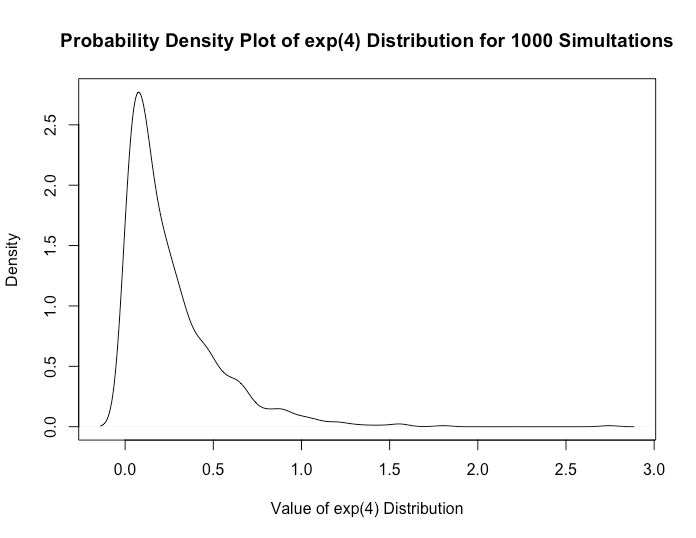
\includegraphics[width=0.6\linewidth]{a1.png}
			\end{center}
		\end{figure}

		The above figure's right tail is longer than the left tail, and the mean sits further to the right than the median, thus the data is right skewed.

		\pagebreak

		\item Using the following code,
		\begin{align*}
			&\code{sim2=replicate(1000,((1/200)*(sum(rexp(200,4)))))}\\
			&\code{densim2=density(sim2)}\\
			&\code{plot(densim2, xlab = }\text{\enquote{\code{Value of each average of 200 exp(4) numbers}}}\code{,} \\
			& \hspace{5mm}\code{main = }\text{\enquote{\code{Probability Density Plot of 1000 Simulations of the Average of exp(4)}}}\code{)}\\
		\end{align*}
		we get the following figure.
		\begin{figure}[h!]
			\begin{center}
				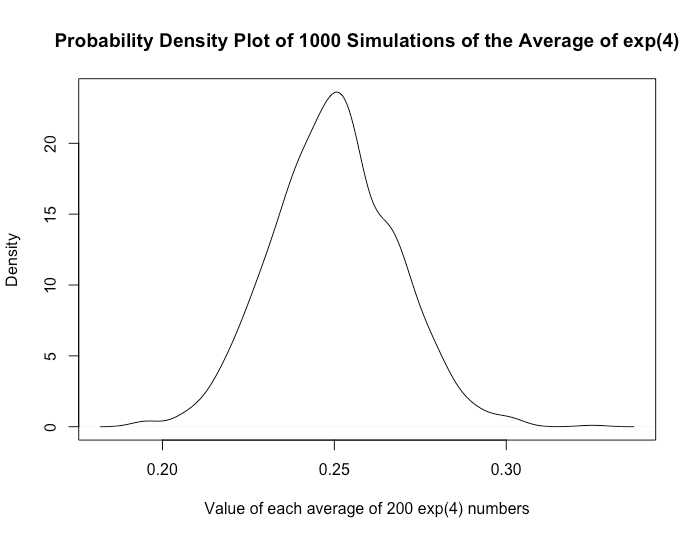
\includegraphics[width=0.6\linewidth]{b1.png}
			\end{center}
		\end{figure}
		\bigbreak
		Using the following code,
		\begin{align*}
			&\code{qqnorm(sim2, main = ,}\text{\enquote{\code{Normal Q-Q Plot of the Simulated Average}}}\code{)}\\
		\end{align*}
		we get the following figure.
		\begin{figure}[h!]
			\begin{center}
				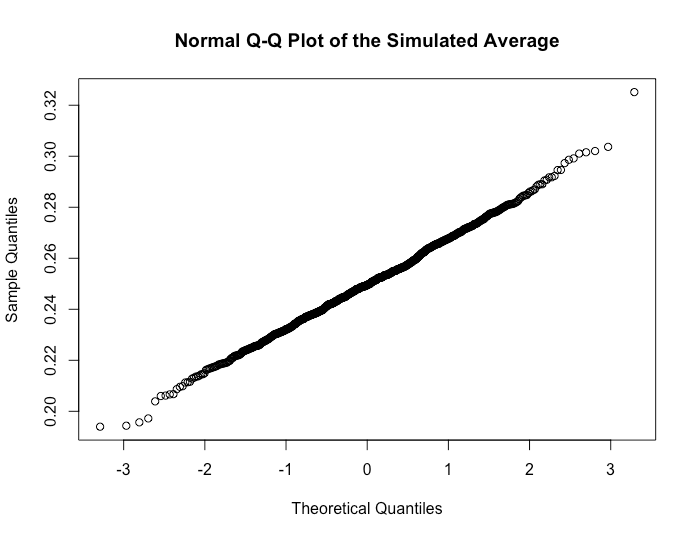
\includegraphics[width=0.6\linewidth]{b2.png}
			\end{center}
		\end{figure}

		\item The Probability Density Plot demonstrates that the distribution of averages of 200 simulations of the exp(4) distribution approximates a normal distribution. In addition, the quantile plot is approximately a straight line, and thus the distribution of the 200 simulations are a linear transform of the normal distribution. This indeed verifies the Central Limit Theorem.

		\pagebreak

		\item Using the following code,
		\begin{align*}
			&\code{sim3=replicate(1000,((1/200)*(sum(rcauchy(200,0,1)))))}\\
			&\code{densim3=density(sim3)}\\
			&\code{plot(densim3, xlab = }\text{\enquote{\code{Value of each average of 200 cauchy(0,1) numbers}}}\code{,} \\
			& \hspace{5mm}\code{main = }\text{\enquote{\code{Probability Density Plot of 1000 Simulations of the Average of cauchy(0,1)}}}\code{)}\\
		\end{align*}
		we get the following figure.
		\begin{figure}[h!]
			\begin{center}
				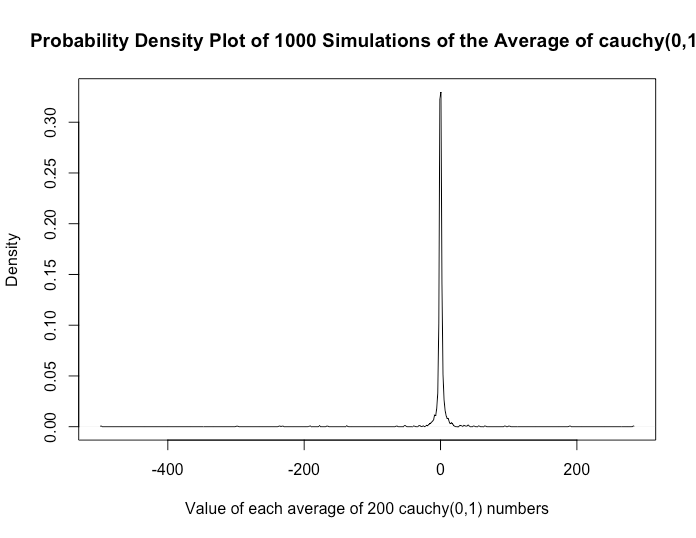
\includegraphics[width=0.58\linewidth]{d1.png}
			\end{center}
		\end{figure}
		\bigbreak
		Using the following code,
		\begin{align*}
			&\code{qqnorm(sim3, main = ,}\text{\enquote{\code{Normal Q-Q Plot of the Simulated Average}}}\code{)}\\
		\end{align*}
		we get the following figure.
		\begin{figure}[h!]
			\begin{center}
				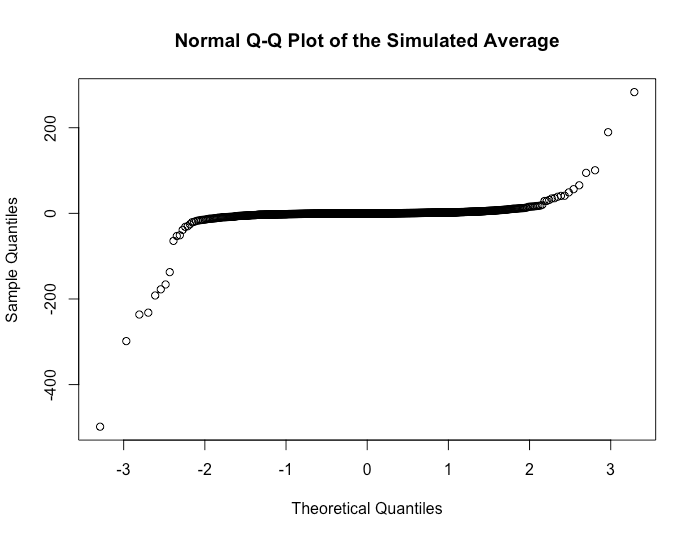
\includegraphics[width=0.58\linewidth]{d2.png}
			\end{center}
		\end{figure}

		\item The distribution of the mean of n independent identically distributed samples from a Cauchy Distribution has the same distribution as the original Cauchy Distribution, regardless of n. Moreover, the probability density plot clearly does not approximate a normal distribution due to its sharp peak and long tails. In addition, the quantile plot does not form a straight line, and thus, the samples from the Cauchy Distribution are not a linear transform of the normal distribution. Thus, the sample mean will never approximate a normal distribution, and in this way, the Central Limit Theorem is not verified.

	\end{enumerate}

\end{enumerate}

\end{document}